% !Mode:: "TeX:UTF-8"

\chapter{图计算相关概念与技术}

\section{图的相关概念}
图是一种复杂的抽象数据结构,能够表示不同物件之间的关系。
%而现实世界的数据量又非常巨大,常规的处理方法难以满足要求,因此需要进行大规模的图计算的研究。
从数据结构的角度出发,图是由有穷非空的顶点集合和表示顶点之间关系的边的集合组成。假如我们使用$G$表示一个图,$V$是图中顶点的集合,$E$表示是图中边的集合,那么一个图就可以表示为:$G=(V,E)$。
在图中,若顶点$Vi$到$Vj$的边没有方向,则这条边是无向边,无向边可以使用无序二元组$(V_i,V_j)$表示。如果图中任意两个顶点之间的边都是无向边,则该图是无向图,而一个图的任意两个顶点之间都有一条边,则称该图为无向完全图;若顶点$V_i$到$V_j$的边有方向,则称这条边为有向边,有向边可以使用有序二元组$(V_i,V_j)$表示,其中$V_i$表示起始顶点,$V_j$称为目的顶点。如果图中任意两个顶点之间的边都是有向边,则称该图为有向图,而有向图中任意两个顶点间都有方向相反的两条有向边,则该有向图为有向完全图。含有n个顶点的无向完全图有$n(n-1)/2$条边,含有n个顶点的有向完全图有$n(n-1)$条边。

在无向图中,一个顶点拥有的边的数量就是该顶点的度。在有向图中,顶点的出度就是以该顶点为起始顶点的边的数量,顶点的入度就是以该顶点为目的顶点的边的数目,该顶点的度为它自身入度和出度之和。在图的边上对其进行标示数字来标示该边的相关的数据信息,则该信息称为边的权重。边上带有权重的图就称为网。

在图中,若存在一系列首尾相接的边组成的顶点序列($V_i$,$V_m$,$V_n$,......,$V_j$)使得从顶点$V_i$到达顶点$V_j$,则称该序列为顶点$V_i$到顶点$V_j$的路径。其中,路径上边的数目就是该路径的长度,若是带权图,则路径的长度是该路径上边的权重之和。若一条路径的起始顶点和终止顶点相同,则称该路径为回路。若路径中只有起始顶点和终止定点是同一定点的路径称为简单回路。否则,没有相同顶点的路径称为简单路径。

如果图$G^0$的顶点和边属于图$G$则称图$G^0$是$G$的子图。在无向图中,如果存在一条从顶点$V_i$到顶点$V_j$的路径,则称顶点$V_i$到顶点$V_j$是连通的。若图中的任意两个顶点都是连通的则称该图为连通图。


\section{常见图算法}
图论作为数学领域中的一个重要分支已经有数百年的历史。人们发现图的许多重要特性,发明了许多重要的算法,其中许多困难问题的研究仍然十分活跃。在解决现实问题时,其他数据结构,例如线性表、树等,都具有明显的条件限制,而图结构中任意两个数据元素间均可相关联。在结构和语义方面,图较之线性表和树更为复杂,但是也更加具有表现能力。因此,现实世界中的数据往往都是以图的结构进行保存。

\subsection{图的存储}
在计算机中,要表示一个图$G=(V,E)$,有两种标准的方法:邻接矩阵和邻接表。这两种方法既可以表示有向图,也可以用来表示无向图。
邻接表表示由一个顶点$V$和以该顶点为起始顶点的边的集合组成。对于图$G$中每个顶点$V$$_i$,把所有邻接于顶点$V$$_i$的顶点$V$$_j$保持为一个单链表,则该单链表称为顶点$V$$_i$的邻接表,如图\ref{fig:graphdemo:adj}所示。邻接矩阵表示的原理就是利用两个数组,其中一个数组用来保存顶点,另外一个数组用来表示边,矩阵中为1的位置表示存在一条边,否则为0,如图\ref{fig:graphdemo:matrix}所示。

另外,图还可以用CSR(Compressed Sparse Row)格式进行保存,CSR格式将顶点\textit{id}和边分别用两个数组进行保存,其中边数组保存边的目的顶点\textit{id}并按照出发顶点\textit{id}排序就,而在顶点数组中顶点的\textit{id}就是数组的索引,每个顶点保存第一条边在在边数组中的索引,如图\ref{fig:graphdemo:csr}所示。
\begin{figure}[htbp]
  \centering
  \subfigure[5个顶点的无向图]{
            \label{ fig:graphdemo:demo)}
            \includegraphics[width=0.2\textwidth]{myfigures/graphdemo.eps}}
  \subfigure[邻接表表示]{
            \label{fig:graphdemo:adj}
            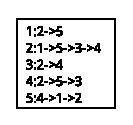
\includegraphics[width=0.15\textwidth,scale=0.5]{myfigures/graphadj.eps}}
  \subfigure[邻接矩阵表示]{
            \label{fig:graphdemo:matrix}
            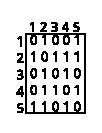
\includegraphics[width=0.1\textwidth,scale=0.5]{myfigures/graphmatrix.eps}}
\subfigure[CSR表示]{
            \label{fig:graphdemo:csr}
            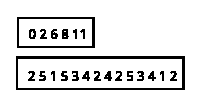
\includegraphics[width=0.2\textwidth]{myfigures/graphcsr.eps}}
  \caption{图的表示方法}\label{fig:graphdemo}
\vspace{\baselineskip}
\end{figure}

\subsection{遍历图}
图的遍历是指从图中给定的某一源点出发,对图中的顶点访问且近且访问一次的操作。图的遍历算法有两种:广度优先和深度优先。

广度优先搜索是最简单的图算法之一,也是很多其他图算法的重要基础。对于给定的图$G=(V,E)$和一个确定的源顶点$s$,广度搜索算法的主要流程如下:
\begin{itemize}
\item 首先访问顶点$s$,并将顶点$s$标记为已访问。
\item 依次搜索$s_0$所有邻接顶点$s_1$,$s_2$,...,$s_m$,并将其标记为已访问。
\item 再按照$s_1$,$s_2$,...,$s_m$的次序依次访问它们的未被访问过的邻接顶点,并将其标记为已访问
\item 以此类推,直到图中所有和源顶点$s_0$有路径相同的顶点都被访问过为止,如图\ref{fig:graphbfs}所示。
\end{itemize}

\begin{figure}[htbp]
\centering
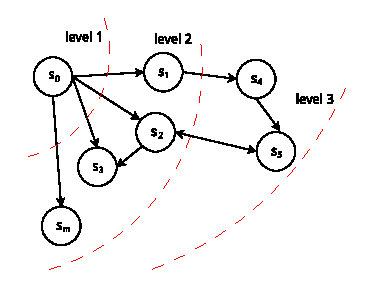
\includegraphics[width=0.4\textwidth]{myfigures/graphbfs}
\caption{广度优先遍历}\label{fig:graphbfs}
\vspace{\baselineskip}
\end{figure}

对于给定的图$G=(V,E)$和一个确定的源顶点$s$,深度优先遍历的基本流程如下:
\begin{itemize}
\item 首先访问顶点$s$,并将顶点$s$标记为已访问。
\item 依次搜索$s_0$的所有邻接顶点$s_i$,若$s_i$没有被访问过,则把顶点$s_i$作为新的源点,继续深度优先遍历,知道图中所有和顶点$s_0$有路径的顶点都被访问一次为止。
\item 如果图中存其他未被访问的顶点,则另选一个作为源点,重复上述步骤,直到所有顶点都被访问过为止,如图\ref{fig:graphdfs}所示。
\end{itemize}

\begin{figure}[htbp]
\centering
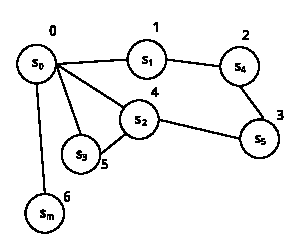
\includegraphics[width=0.4\textwidth]{myfigures/graphdfs}
\caption{深度优先遍历}\label{fig:graphdfs}
\vspace{\baselineskip}
\end{figure}

\subsection{单源最短路径}



\subsection{最小生成树}

\subsection{PageRank}

\section{大规模图计算技术}

大规模图对象,顶点与边的数目都非常巨大,难以全部载入内存进行处理。由于图的算法往往呈现出一定的随机性,而这种情况在大规模图中表现的更为明显,给传统的需要一次性将图载入内存的应用带来巨大的挑战。例如,顶点$V_i$存在某一条<$V_i$,$V_j$>,由于该图比较大,顶点$V_i$以其相关的边已经载入内存中,而顶点$V_j$却还存在于磁盘上,此时对该图进行遍历,需要访问顶点$V_j$,则需要访问磁盘读入顶点$V_j$的相关信息,在这样的情况下传统图处理算法就会因为不得不频繁的访问磁盘而造成处理效率极度低下。另外,图的有些算法是递归实现的,对于大规模的图,这种实现很容易出现无限递归调用的情况。所以,对于大规模图的处理无论是可行性还是计算效率,传统的算法实现都不适用,所以需要研究能够用来处理大规模图对象的框架和算法。

目前,针对大规模图处理已经存在一些分布式和单机上的解决方案,例如,Pregel、GPS、Mizan、GraphChi以及X-Stream等。虽然这些解决系统各自的实现方式细节不同,但是总的来说,对于大规模的图处理技术而言,目前主要分为两种:以顶点为中心的计算模型和以边为中心的计算模型。

\subsection{Vertex-Centric模型}
顶点为中心的大规模图处理模型由谷歌在Pregel系统中提出。在以顶点为中心的计算模型中,顶点是整个计算的核心,每个顶点保存着图处理中的主要信息,顶点之间互相发送各自的更新消息,并且顶点可以根据接受到来自其他顶点的消息对其进行计算并更新自己的消息。同时顶点有两个状态:激活和未激活。当顶点接收到消息的时候,顶点就处于激活状态,否则处于未激活状态。当所有顶点都处于未激活状态的时候,计算完成,如图\ref{}所示。以顶点为中心的计算模型非常适合大规模的图处理,这主要是因为虽然图处理的整体计算很多,但是具体分到每个顶点的计算量非常少,同时无需关心顶点是否存在于内存中或者是否存在于本地或者存在于其他计算节点。在实现以顶点为中心的计算模型中,用户只需要实现每个顶点如何处理消息的方法即可,极大地简便了基于大规模图的应用开发。
例如,如果要实现一个基于以顶点为中心的最短路径算法,首先指定一个源顶点$V_0$,顶点的值表示从源顶点到某一个顶点的距离,那么源顶点的值初始化为0,其他初始化为无穷大;然后从源顶点开始将自身的值封装为消息,并发送给它的邻接顶点,其他顶点接收到消息后,将消息与自身的顶点值进行比较,若消息值较小,则将消息值加1后作为自己新的顶点值,然后并将该更新状态发送给其他顶点。否则,不做任何处理。当图中所有顶点都不在更新状态,即所有顶点都处于未激活状态,那么计算结束。

\subsection{BSP计算模型}
Vertex-Centric模型从理论上极大地简化大规模图处理过程。但是这种没有控制的随意消息发送方式只能处理简单的图应用算法,由于需要发送和产生大量的消息,对于没有载入内存的顶点而言,或者消息的接受顶点存在于远程计算节点上,就需要对大量的消息进行缓存,这样由于需要IO操作或者通讯延迟而造成的状态消息更新速度不匹配,很可能造成某些顶点的重复计算。例如,对于一个最短路径算法而言,某个顶点因为存在于内存中,它处理的消息更新迭代可能远远高于保存在磁盘上或者远程计算节点上的顶点。而对于一个基于以顶点为中心的PageRank算法,一次迭代是需要严格的消息更新状态的,在没有同步的控制下,难以保证正确性,同时容易造成消息风暴。
所以为避免这样的问题,将以顶点为中心的大规模图处理过程,分为一系列连续的超级步,每个超级步结束时同步,并完成对消息的发送和缓存等操作,该模型就是BSP计算模型。

BSP是Bulk Synchronous Parallel的缩写,是一个通用的并行计算模型,最初作为一个并行计算领域中软件和硬件之间的“过渡模型”而提出的。BSP,“大块”同步模型,其概念由哈佛大学的Valiant和牛津大学的Bill McColl提出,支持消息传递,块内异步并行,块间显式同步。BSP一般由三个部分组成:处理的任务单元、任务单元之间的消息通讯和对全局任务单元进行全局同步的机制,如图所示。BSP模型非常适合分布式的图计算环境。首先,BSP模型具有全局的数据通信网络。BSP中的各个处理单元和通过它和其他处理单元进行通信或内存的存取,这和大多数基于分布式内存或消息传递的并行模型是相同的。不同的是BSP的通信是一个全局的概念,不是点对点的通信,能够很好的解决图计算过程中数据的随机访问问题。其次,BSP模型具有全局的路障同步机制。路障同步的引入则能保证图处理过程的完整性,提高整个图处理的鲁棒性和可靠性。因此,很多基于分布式内存的大规模图处理统都构建在BSP模型的基础上,例如Pregel、GPS等。

在BSP模型中,任务单元负责对分配给它的大规模图的顶点进行循环遍历,并调用消息处理函数,然后将顶点的更新消息发送给其他顶点。从顶点的角度而言,图的处理过程由两个过程组成:顶点调用消息处理函数计算消息和发送自身的更新状态。如此迭代,直到所有任务单元完成对顶点的遍历以及函数调用和消息发送过程,在全局路障处同步,当前超级步完成,所有任务单元进入下一个超级步。

\subsection{Edge-Centric模型}
以边为中心的计算模型与与顶点为中心的计算模型较为类似,但是殊途同归并且本文不以该模型为重心,所以不做过多赘述仅对该模型进行必要的介绍。如图\ref{fig:evc}所示首先,该模型对边进行遍历,并且通过边将消息发送出去;然后,对边上的目的顶点进行更新。与以顶点为中心不同,以边为中心的计算模型将计算根据边分为Scatter和Gather两个阶段,在Scatter阶段对边进行读取,然后将边的起始顶点的信息通过边发送给目的顶点;在Gather阶段,同一将Scatter阶段的消息进行处理更新。

\begin{figure}[htbp]
\centering
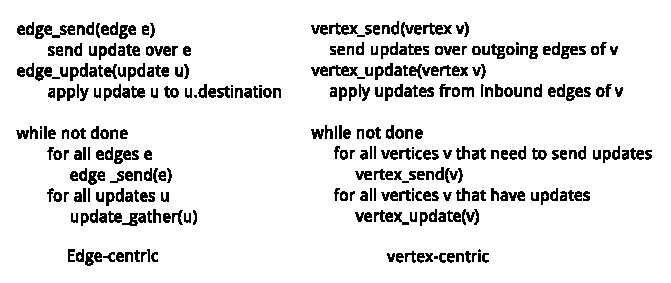
\includegraphics[width=0.6\textwidth]{myfigures/edgevertexcentric.eps}
\caption{以边为中心和以顶点为中心的算法流程}\label{fig:evc}
\vspace{\baselineskip}
\end{figure}

\section{大规模图处理中的并发}

大规模图对象因其数据量之庞大,传统的顺序的完全载入内存的方式不适合处理大规模图对象。如果需要将所有图都载入内存当中进行计算,就需要使用分布式的计算资源,将图分为若干部分,均衡的分配给每一个计算节点。同时不同的计算节点之间需要互相通讯以交换数据。在前文中我们介绍了大规模图计算中使用的主要技术:以顶点为中心的计算模型和BSP并发模型。在本节将会解释在大规模图计算中使用的并发技术。


随着计算机多核处理器的出现和内存不断增大,单台计算机的计算性能实际上已经有着很大的提升。
在过去40多年时间里,计算机性能一直遵循着摩尔定律,集成电路上可容纳的晶体管数目,约每隔18个月便会增加一倍,而集成电路的性能(计算能力)也将提升一倍。近年来,集成电路的集成程度已经非常高,芯片上元件的几何尺寸不可能无限制的缩小下去,摩尔定律面临挑战,遭遇瓶颈。另外,仅仅提高单核芯片的速度会产生过多的热量并且无法带来相应的性能改善。然而,人们对于电脑的要求不断提高,迫使处理器向高性能的方向发展。如果多一颗同一性能的处理器,理论上处理能力是原来的两倍。于是,为了进一步提高性能,就需要更多的处理器,将多个处理器置入单一芯片中,构成多核心处理器。于是,有相关学者和研究人员提出基于单机共享内存的图处理系统,例如GraphChi、X-Stream等。实验证明,这些单机上图处理系统经过严谨而合理的设计不仅具有高效便捷的优势,还能大大的降低开发成本。但是,随着网络的发展,数据量的海量递增趋势已经越来越明显,现有的一些单机系统在扩展性上很难满足这样的挑战。目前应用于企业级的图处理系统大部分仍然基于BSP模型的分布式系统,而现有单机系统往往从系统IO优化处着手,两者之间很难互相兼容。另外,局限于目前多核的并发编程理论并不成熟,造成单机环境下多核计算机的计算能力并没有被充分利用。传统上的单机多核并行软件开发往往是基于共享内存的,共享内存就很容易引起竞争条件,为保证程序的准确性和一致性,就必须对可能引起竞争的变量或者语句进行加锁保证互斥或者进行同步。此外,从硬件层面考虑,多核虽然提高了计算性能,但是随着核数的增多,核与核之间也会出现消息通讯,内存数据一致性等问题.

常见的图算法有遍历、最短路径、最大连通分量等。对于规模较小可以完全载入内存的图,单线程的处理方式需要顺序依次对顶点进行遍历访问即可。但是,当图的规模巨大时,这种单线程的执行方式就难以满足需求。大规模图的处理技术同时具有IO密集型和计算密集型两种特点。IO密集型是因为大规模图对象数据量庞大,无法一次性全部载入内存进行计算,同时还会涉及大量的中间结果的读写。而计算密集型则是因为基于大规模图对象的应用需要对整个图进行分析计算,涉及大量的迭代和计算。因此,传统的单线程的开发方式不仅能造成IO阻塞降低图处理的效率,还无法充分发挥多核计算机的有事,造成计算资源的浪费。因此,对于大规模图对象的处理一般采用并发的方式来提高图处理的效率。

为了能够更加有效的利用硬件所提供的性能,传统的应用开发方式现在已经不适用了。以往的应用开发方式在大部分情况下所面对的都是只有一个单独的处理器,也就是意味着顺序执行的单线程应用。如今,多核计算机逐渐成为主流配置,并且价格也在不断地降低。而要处分发挥多核计算机的计算能力,最简单的办法就是利用并发,编写能够在多个核心上运行的任务,并且任务之间可以通过共享数据的方式进行通信协同工作,也就是并发程序。

为适应当今社会多核的迅猛发展,许多并发模型应运而生。在JVM平台上,已经存在的并发模型有传统同步模型、软件事务内存模型和角色模型三种。目前,实现并发程序有许多方式,以操作系统的支持,可以用进程,或是线程。以编程语言的支持,在JVM平台上可以使用多线程,JDK并发模型、软件事务内存、基于角色的并发模型。


\section{多线程在图计算中的应用}



首先,大规模图一般情况无法完全载入内存,需要分批依次载入并进行计算处理。这样图的处理就会涉及大量的IO读写操作,单线程程序会引起IO阻塞,不仅降低图的处理效率。其次,对于操作系统而言,线程是基本的调度单位,在双处理器的计算机上,单线程的程序只能利用一半的CPU资源,造成计算资源的浪费。而如果采用多线程的方式,




由于基本的调度单位是线程,因此如果在程序中只有一个线程,那么最多同时只能在一个处理器上运行。在双处理器系统上,单线程的程序只能使用一半的CPU资源,而在拥有100个处理器的系统上,将有99$\%$的资源无法使用。如果仍然按照传统的开发方式,多核的优势就无法发挥,对计算资源造成浪费。
另一方面,多线程程序可以同时在多个处理器上执行。如果设计正确,多线程程序可以通过提高处理器资源的利用率来提升系统吞吐率。使用多个线程还有助于在单处理器系统上获得更高的的吞吐率。如果程序是单线程的,那么当程序等待某个同步I/O操作完成时,处理器将处于空闲状态。而在多线程程序中,如果一个线程在等待I/O操作完成,另一个线程可以继续运行,使程序能够在I/O阻塞期间继续运行。




\section{Actor模型简介}

角色模型是一种不同的并发进程建模方式。与通过共享内存与锁交互的线程不同,角色模型利用了 “角色” 概念,使用邮箱来传递异步消息。在这里,邮箱类似于实际生活中的邮箱,消息可以存储并供其他角色检索,以便处理。邮箱有效地将各个进程彼此分开,而不用共享内存中的变量。

角色充当着独立且完全不同的实体,不会共享内存来进行通信。实际上,角色仅能通过邮箱通信。角色模型中没有锁和同步块,所以不会出现由它们引发的问题,比如死锁、严重的丢失更新问题。而且,角色能够并发工作,而不是采用某种顺序方式。因此,角色更加安全(不需要锁和同步),角色模型本身能够处理协调问题。在本质上,角色模型使并发编程更加简单了。

角色模型并不是一个新概念,它已经存在很长时间了。一些语言(比如 Erlang 和 Scala)的并发模型就是基于角色的,而不是基于线程。实际上,Erlang 在企业环境中的成功(Erlang 由 Ericsson 创建,在电信领域有着悠久的历史)无疑使角色模型变得更加流行,曝光率更高,而且这也使它成为了其他语言的一种可行的选择。Erlang 是角色模型更安全的并发编程方法的一个杰出示例。


\section{Kilim简介}

Kilim是一个使用JAVA编写的并发库,融入了角色模型的概念。Kilim由一个称为Weaver的后期进程来实现,该进程转换类的字节码。包含 Pausable throws 字句的方法在运行时由一个调度程序处理,该调度程序包含在 Kilim 库中。该调度程序处理有限数量的内核线程。可以利用此工具来处理更多的轻量型线程,这可以最大限度地提高上下文切换和启动的速度,并且每个线程的堆栈都是自动管理的。但是,Kilim设计之初并没有考虑到大量的协程之间的消息通讯,所以Kilim在面对频繁大量的协程通讯显得力不从心。

Disruptor[31]是一个开源的应用在Java平台上的低延迟高吞吐量的并发框架。LMAX是一种新型零售金融交易平台,Disruptor是LMAX的一个业务逻辑处理器,它能够在一个线程里每秒处理6百万订单,它完全运行在内存中,使用事件源驱动方式。在Disruptor框架中避免锁机制,添加缓存行填充来消除伪共享,以此提高并发性。但是,Disruptor的框架适用于线程,并且局限于特定平台。
因此,我们的工作主要围绕两个方面进行:1)、高并发编程的以顶点为中心的单机模型;2)、单机多核环境下高效的消息传递机制。


\section{小结}